\section{Design analysis and controlled ablations}
\label{sec:design-analysis}
Three findings shaped PHASE-TTC: preserving scale change mattered more than representation stability alone; correcting an expert's phase could improve on selecting an expert; and changing the loss often traded one TTC range against another. The studies below used different data splits and pretrained models. Appendices~\ref{sec:early}, \ref{sec:temporal-recovery}, and~\ref{sec:late} give the full configurations and unsuccessful variants.

\subsection{Preserve the motion variable before predicting it}
Using a common object region preserves apparent expansion across observations. Independently resizing each endpoint can remove that signal before the network sees it (Figure~\ref{fig:crop}). An explicit object query also distinguishes objects that share one full-frame input but have different TTC targets. The estimator consequently requires externally supplied localization. \evidence{M03}

The synthetic experiments showed why embedding stability alone was insufficient. With slowly changing nuisance features, a temporal-residual objective recovered more dynamic information than a variance regularizer. Changing those nuisance features independently every frame reversed the ordering. The geometry experiments exposed a related difficulty: stable foreground maps and accurate absolute heights did not ensure accurate changes in scale. Some models also received RGB-derived SAM masks or DINOv3 relations during training, even when their inference inputs contained only events. \evidence{E02,E12,E25,E26}

Removing paths from a trained V8 model identified which inputs its prediction used. Analytic scale alone scored 373.18 MiD, and adding the residual without transport gave 373.60. Restoring transport reduced the score to 163.23; restoring history reduced it further to 155.82. The weights remained fixed throughout these tests. Separate JEPA controls did not establish a benefit from predictive pretraining. \evidence{E21,E23,E24}

\subsection{Correct phase rather than only selecting an expert}
A hard router is limited to the predictions its experts already make. SIMPLEX-T can move beyond them by learning a correction around their median phase from masked temporal context. The auxiliary cost head still describes the original experts, so it does not directly estimate the corrected prediction's risk. The phase quantiles likewise require calibration before they can be interpreted as collision probabilities. \evidence{M_TEMPORAL_MODEL,M_PHASE_CONTRACT}

Extending history from H8 to H16 lowered MiD for each of three head seeds on OLD\_DEV. The paired interval across all seeds excludes zero. However, one seed had already informed exploration; the two new seeds alone give a difference of $-2.42$ MiD with interval $[-5.24,0.04]$. All heads shared the same upstream producers. Figure~\ref{fig:main-h16} shows both summaries; H8 remained the selected candidate. \evidence{M_SIMPLEX}
\begin{figure}[htbp]
\centering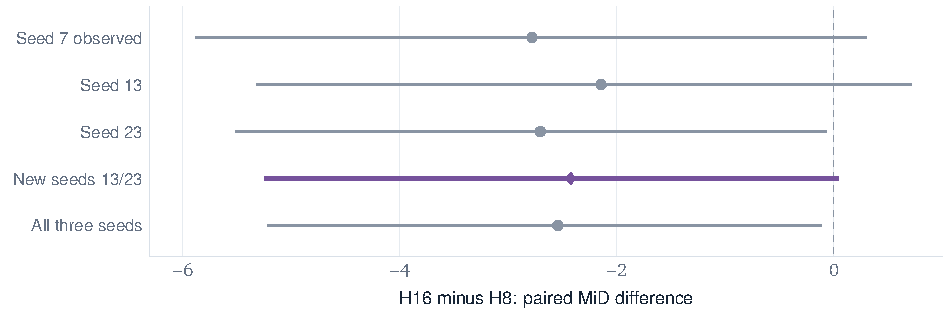
\includegraphics[width=.97\linewidth]{figures/rev_h16.pdf}
\caption{\textbf{H16 minus H8 on nine OLD\_DEV sequences.} Points show paired MiD differences and lines show the recorded hierarchical 95\% intervals. The highlighted estimate uses only the two new head seeds; its interval includes zero. \evidence{M_SIMPLEX}}
\label{fig:main-h16}
\end{figure}

Keeping all experts produced the lowest score in the removal study: FULL-C0 reached 121.40 MiD, compared with 127.79 for A5-only, 126.70 for C2F-only, and 124.67 for A5 plus PAIR. \evidence{M_SIMPLEX}

In the temporal-aggregation comparison, set aggregation with age gave 122.44 MiD; removing explicit time gave 123.69. Because the frozen experts can already encode temporal information, the remaining differences cannot be assigned to recurrence alone. \evidence{M_X05}

Transport probes improved on destructive controls, but stronger calibrated or pooled alternatives narrowed that advantage. \evidence{M_STAGE61,M_STAGE62}

\subsection{Adaptation trades error between TTC ranges}
Changes to the readout often improved imminent-contact estimates at the expense of receding motion. V14 M1--L0 reduced crucial MiD from 156.83 to 134.47 but increased negative MiD from 61.38 to 84.21. V17's geometry bypass lowered the aggregate score on the development-used V split from 106.545 to 102.762 while worsening MAE; its head seeds shared encoders. Across V14--V17, loss reweighting, residual range, sampling, numerical precision, clipping, geometry bypasses, and height readouts failed to meet all acceptance criteria. Invalid height-derived predictions were retained in scoring. The next experiments therefore allowed the measurement model itself to adapt. \evidence{L02,L50--L52}

V18 full adaptation reduced aggregate MiD on H from 112.29 to 78.92 and crucial MiD from 157.27 to 95.85, while negative MiD rose from 65.52 to 87.09. The model passed the overall sign criterion but remained inaccurate in the magnitude of receding TTC. V19 increased the training weight on negative targets and recovered some negative-range accuracy and MAE, at the cost of aggregate and crucial-range error. \evidence{L10,L24,L25,L30}

\subsection{Events help in the matched V18 comparison}
Supplying real events improved V18 C1 relative to its equal-capacity ZERO control. TRUE-event fusion achieved aggregate MiD $87.29\pm0.87$, compared with $92.47\pm0.16$; dispersion is the sample standard deviation of the scalar scores across seeds. The paired comparison over complete groups also favored TRUE. Each seed repeated C1 adaptation and head fitting from the same A5 initialization and RGB context model. This experiment uses V18 C1, whereas the final TRAIN40 system derives from V16. \evidence{L03,L31--L33}
\begin{figure}[htbp]
\centering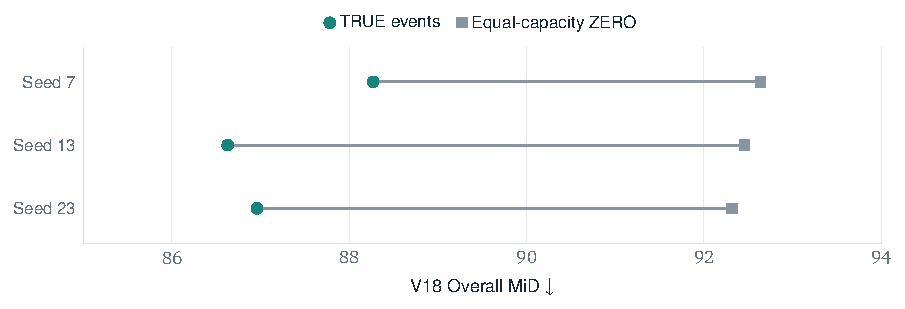
\includegraphics[width=.97\linewidth]{figures/rev_v18.pdf}
\caption{\textbf{Real versus zeroed events in V18 C1.} Each line pairs TRUE and ZERO scores for one adaptation/head seed. The models share the A5 initialization and RGB context model, and TRUE uses the observed event features. \evidence{L03}}
\label{fig:main-v18}
\end{figure}

The V18 crucial-band gain remained below its registered threshold. Its comparison with the preserved V16 model gave an interval of approximately $[-3.69,0.14]$, and no V18 candidate met all acceptance criteria. Testing ZERO events and equal temporal support in the final TRAIN40 recipe would be needed to extend the attribution result to the submitted system.
\FloatBarrier
